\documentclass{beamer}
\usepackage{presentation}

\begin{document}

\frame{\titlepage}

\begin{frame}
  \frametitle{Need and goal statement}

  What we
  \textbf{need}:
  \input{build/need_statement_md}
  \newline
  \newline
  Our
  \textbf{goal}:
  \input{build/goal_statement_md}

\end{frame}

\begin{frame}
  \frametitle{Design Objectives}

  Four key objectives:
  \begin{itemize}
    \item Presence
    \item Portability / ease of set-up
    \item Configurable
    \item Accessible
  \end{itemize}

\end{frame}

\begin{frame}
  \frametitle{What our project could have been...}

  Map task management methods to devices, generate unique ideas
  \newline
  \newline

  \begin{columns}
    \column{0.5\textwidth}
    Method
    \begin{itemize}
      \item Personal assistant
      \item Accountability
      \item Streaks, levels
      \item Planner
    \end{itemize}

    \column{0.5\textwidth}
    Device
    \begin{itemize}
      \item Home assistant
      \item Face tracking sprayer
      \item Game device
      \item PDA Device
    \end{itemize}

  \end{columns}

\end{frame}

\begin{frame}
  \frametitle{Choosing the best design}

  We derived weights from our daily use of electronics and apps

  \begin{longtable}[]{@{}ll@{}}
  \toprule
  Criteria & Weight \\
  \midrule
  \endhead
  Budget & 20 \\
  Presence & 20 \\
  Ease of Use & 20 \\
  Barrier of Entry & 20 \\
  Sustainability & 10 \\
  Privacy & 10 \\
  \bottomrule
  \end{longtable}

  \note[item]{Explain what each of these mean}
  \note[item]{Connect weights with decision chart}
  \note[item]{Show how these weights apply to the products shown in the previous slide}

\end{frame}

\begin{frame}
  \frametitle{Embedded System Flow}

  \begin{center}
    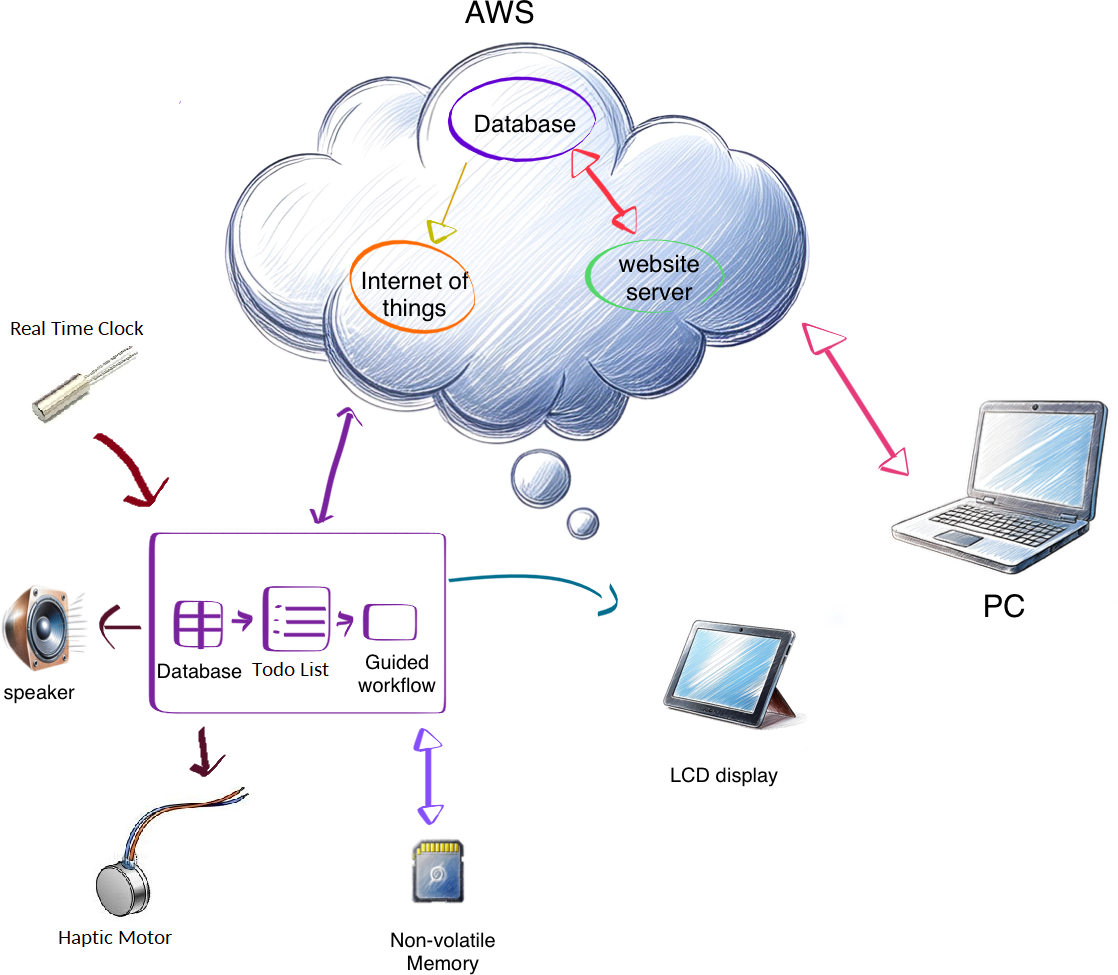
\includegraphics[height=0.7\textheight]{embedded_system_flow_chart.png}
  \end{center}

  \hfill {\tiny Source: Apple Playground for images}

  \note[item]{AWS IoT provides MQTT connection with esp32}
  \note[item]{Simple Storage Service (S3) provides database}
  \note[item]{Elastic Compute Cloud (EC2) provides web server}
  \note[item]{Web server with Flask + boto3 (S3 SDK) on python, nginx for the actual server, all on docker}
  \note[item]{Audio, LCD, and storage will be managed by their own components}
  \note[item]{Everything will be running as a FreeRTOS task with some shared resources}

\end{frame}


\begin{frame}
  \frametitle{Testing}

  \begin{columns}
    \column{0.7\textwidth}
    Testing on the microcontroller can be automated with Unity and pytest.
    \newline
    \newline
    For physical and software tests, we will define the following:
    \begin{itemize}
      \item Stimulus
      \item Control variables
      \item Expected Results
      \item Walkthrough of the procedure
    \end{itemize}

    \column{0.3\textwidth}
    
\includegraphics[width=0.5\textwidth]{pytest_logo.png} \\
    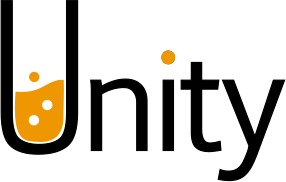
\includegraphics[width=0.5\textwidth]{unity_logo.png}

  \end{columns}

  \hfill {\tiny Source: pytest docs, Unity homepage}
  \note[item]{Unity for unit testing functions}
  \note[item]{pytest for automating tests on the target}
  \note[item]{Mention testing for areas outside areas defined by software - durability, user experience, etc.}
  \note[item]{Any automated tests performed on the software will be done using pytest and Unity. pytest is capable of running automated tests on individual components of the esp32c3 while unity can run any tests that don't require a driver, so it doesn't require the usage of the esp32 for testing.}
  \note[item]{we can design a variety of tests on for example, expected outputs when the user makes a choice. If the user chooses to delay a task, we can directly compare the output of a task checker function against expected values. These tests can be automated and repeated multiple times. This is especially useful when combined with the ESP ERROR output values.}
\note[item]{checking user data persistence on the sd card}
\note[item]{visual inspections to ensure lcd connectivity and functionality}
\note[item]{checking the implemented scheduling algorithm to see if it's displaying what's expected}
\note[item]{stress testing the algorithm by creating impossible schedules or very complex schedules}
\note[item]{testing internet connectivity}
\note[item]{ensuring data is consistent between both the cloud database and the device}
\note[item]{restoration from a cloud backup in the event of sd card corruption or full system failure.}
\note[item]{persistent data display when not connected to the cloud. although this device can sync to the cloud so someone can check their phone for more information, this device can also be brought to discourage someone from relying on their phone as much.}
\note[item]{modularity testing, in the event a part is broken and the user could possibly send their unit in for repair, we want to ensure data and user settings are fully restored from the sd card}
\note[item]{checking encryption to ensure data is fully encrypted end to end and is still decryptable via a replacement device}
\note[item]{strength checks to ensure the body is durable enough to not be bent.}
\note[item]{begin with 1/2 foot drop tests to ensure the body does not instantly break as this is intended to be somewhat portable}
\note[item]{chemical tests, we've discussed some more ecofriendly packaging, but it's important to check what chemicals the device may be sensitive to.}
\end{frame}

\begin{frame}
  \frametitle{Prototype}

  \begin{center}
    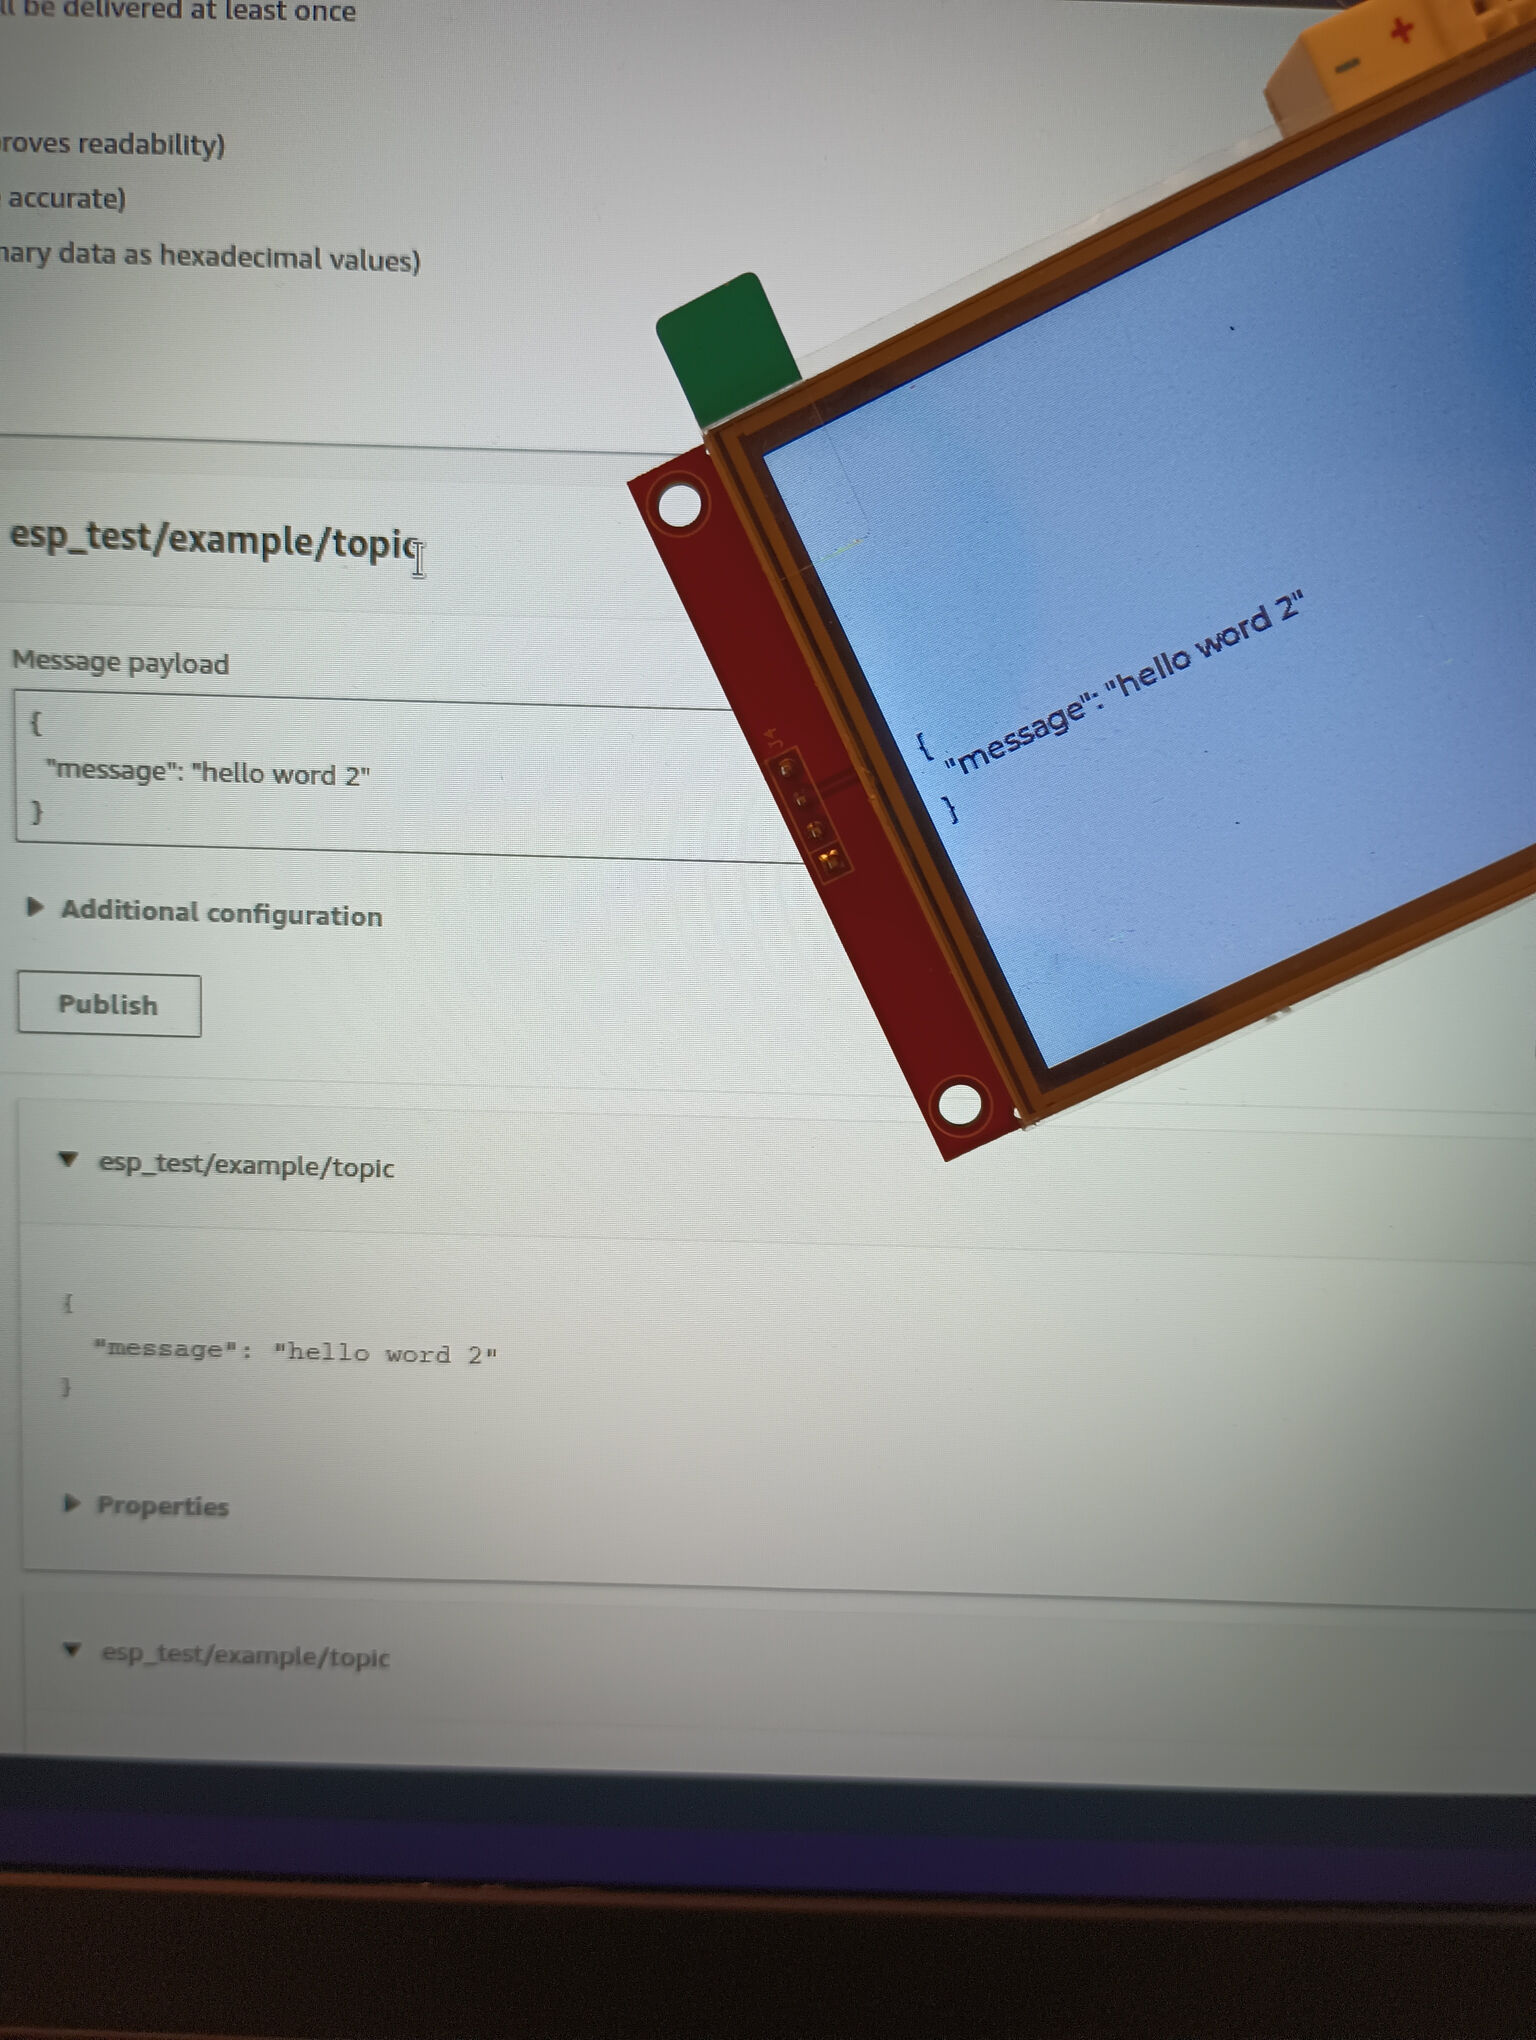
\includegraphics[height=0.7\textheight]{aws_demo.jpg}
  \end{center}

\end{frame}

\begin{frame}
  \frametitle{Algorithm Overview}
  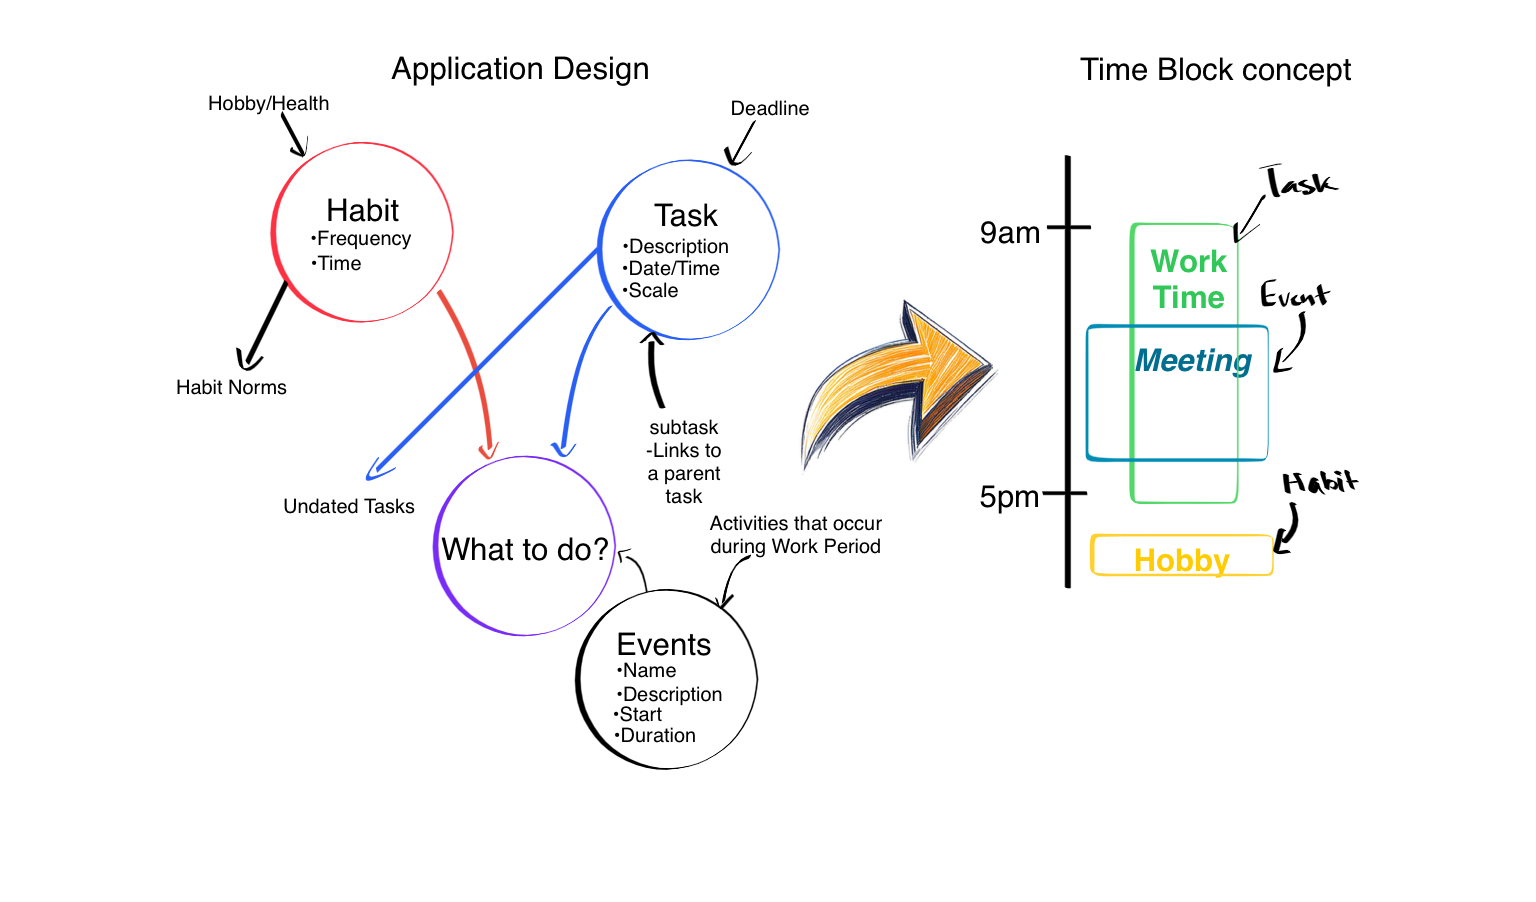
\includegraphics[width=\textwidth]{design_logic.png}

  \note[item]{The system focuses on what the user should currently be doing, focusing on there here and now.}
  \note[item]{3 main entry types: Tasks, Habits, and Events:}
  \note[item]{\textbf{Tasks:} An objective that must be completed by a target date.}
  \note[item]{\textbf{Habbit:} A task that is consistently repeated.}
  \note[item]{\textbf{Event:} A period of time the user is occupied.}
  \note[item]{Time blocks add a reference for our timeless logic. Dictated by the user, these begin guided work sessions where the user is fed the tasks in order from most priority to least priority, given a choice between highest priority items.}
\end{frame}

\begin{frame}
  \frametitle{What's next?}
  % Confidence on on-time completion
  \begin{itemize}
    \item Unit testing with each module
    \item Database management software
  \end{itemize}
\end{frame}

\end{document}
